\section{作业及答案：结构力学基础与技巧班第15次作业及答案（动力学）}
\begin{analysisbox}
动力学题先明确自由度和广义坐标，建立质量、阻尼、刚度关系。单自由度系统重点掌握固有频率、阻尼比和动力系数。
\end{analysisbox}
\subsection*{第 1 页转写}
十一、练习题

1.基本概念

9-1设直杆的轴向变形不计，图9-63所示体系的动力自由度为（

）。（合肥工业

大学2009)

A. 1

C. 3

B. 2

D. 4

9-2设直杆的轴向变形不计，图9-64所示体系的动力自由度为

。（合肥工

业大学2006)

图9-63

图9-64

9-3

图9-65所示结构，其动力自由度个数为

。（西安建筑科技大学2011)

9-4判断题。结构的自振频率、振型都反映结构本身固有的动力特性。（

）（中南

大学2009)

9-5结构的振动自由度是指确定结构的

，所需的独立几何参数数目。（

（中南大学2011)

A.全部结点位置

B.全部杆件的位置

C.全部质点的位置

D.全部动力荷载作用点的位置

9-6单自由度结构的自振频率随刚度的增大而

（增大，减小），随质量的增

大而（增大，减小）。（北京科技大学2010）

9-7判断题。图9-66（a）所示体系的自振频率比图9-66（b）的小。（

）（西

南交通大学2009)

(g)

(b)

图9-65

图9-66
\begin{figure}[H]\centering
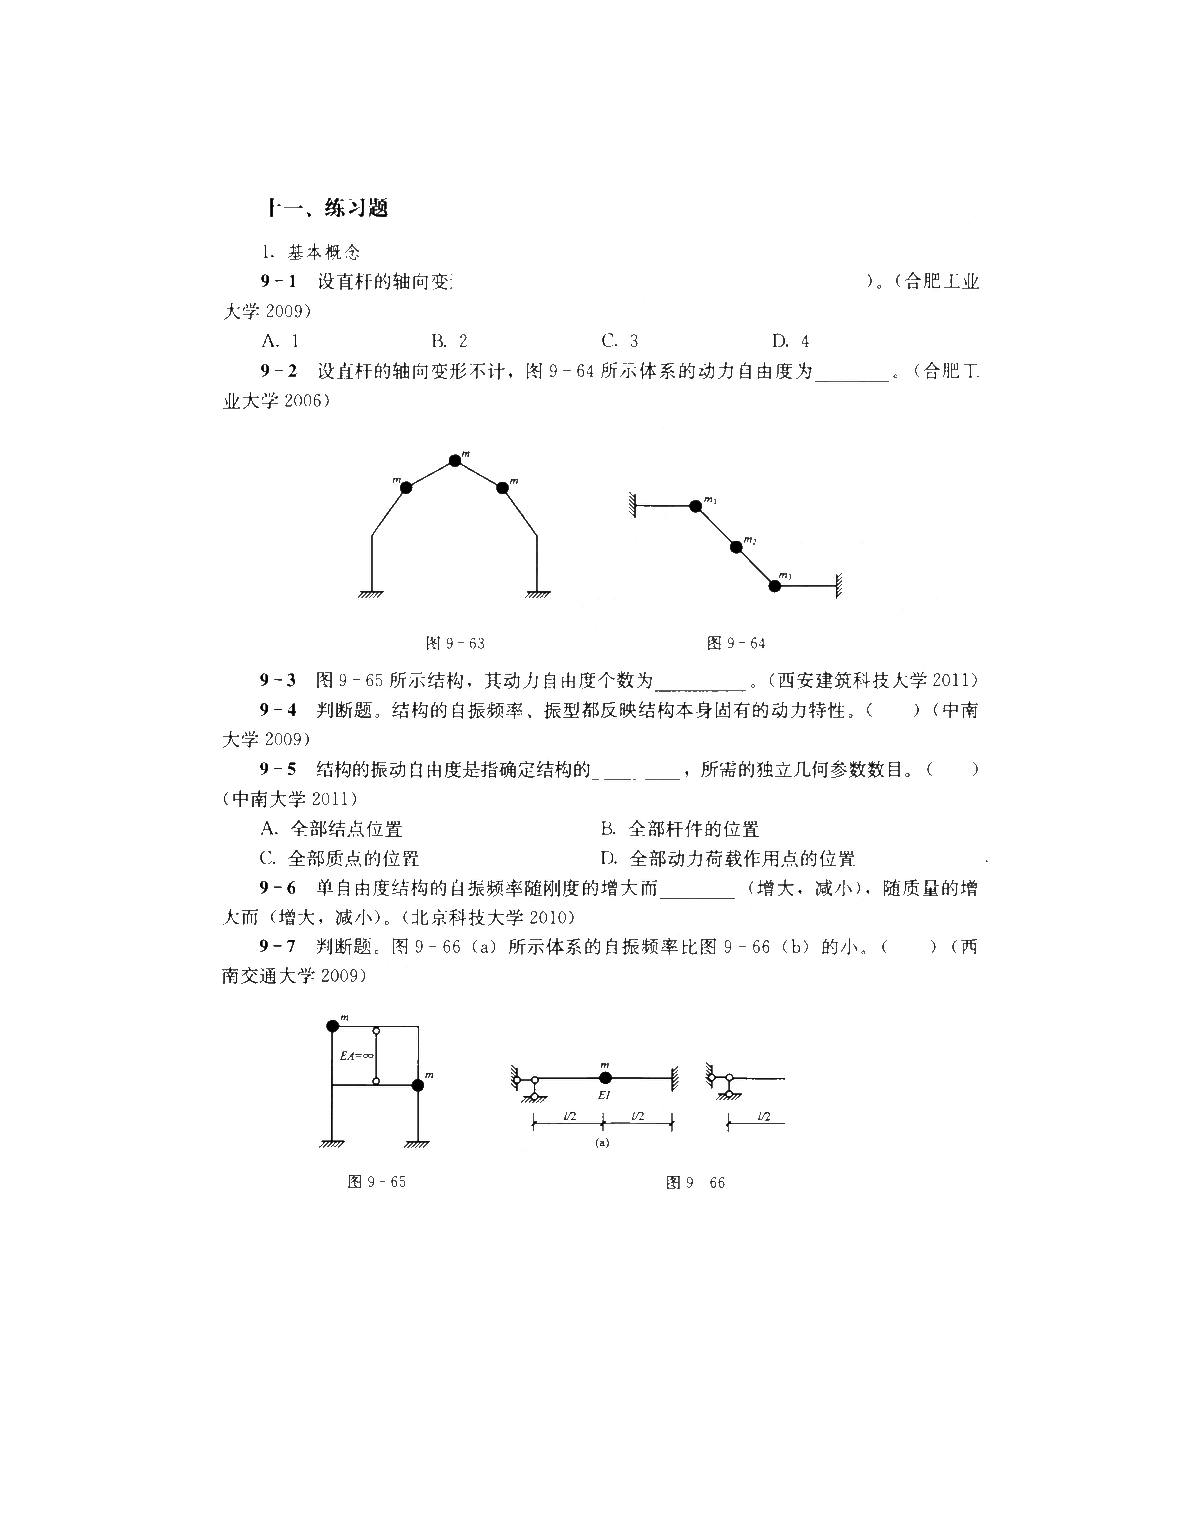
\includegraphics[width=0.92\textwidth]{figures/src18_p001.jpg}
\caption{结构力学基础与技巧班第15次作业及答案（动力学） 第 1 页清理图形页}
\end{figure}
\subsection*{第 2 页转写}
9-8判断题。对于单自由度体系，体系的内力和位移有统一的动力系数。（

）（福

州大学2012)

9-9判断题。体系的动力系数一定大于1。（，）（福州大学2011)

9-10使单自由度体系的阻尼增加，其结果是（

）。注：阻尼增加后仍是小阻尼

（西南交通大学2009)

A.周期变长

B.周期不变

C.周期变短

D.周期视具体体系而定

9-11

阻尼力与质点速度大小成

（正比，反比），方向相反；惯性力与质点加

速度大小成

（正比，反比），方向相反。（北京科技大学2010）

9-12下列叙述正确的是（

）。（西安建筑科技大学2008）

A，位移法是求解超静定结构的基本方法，不能用来求解静定结构

B.阻尼使体系的自振频率变大、使自振周期缩短

C.阻尼使体系的自振频率变小、使自振周期延长

D.力法是求解超静定结构的基本方法，也可用来求解静定结构

2.单自由度体系的计算

9-13已知图9-67中结构集中的重力G（单位为kN）位于D点，梁结构集中重力处

D点作用一简谐荷载F（t)=Fpsin(ot），其中Fp=2kN，Q=0.7w。EI为常数。计算梁结构

的自振频率、周期及D点处最大竖向动位移。（忽略阻尼的影响）（青岛理工大学2011）

9-14计算图9-68中结构的竖向自振频率、周期及绘制动弯矩幅值图（不计水平自

由度影响）。已知结构集中的重力G（单位为kN）位于D点，结构内B点作用一简谐荷载

F（t)=Fpsinat，其中Fp=5kN，Q=0.8w，EI为常数。（不计阻尼的影响）（青岛理工大学

2012)

IFr(0)

EI

3m

2m

4m

im+

+2m+2m

图9-67

图9-68

9-15已知图9-69中m=3t，Fp=8kN，千扰力转速为150r/min，不计杆件质量，

EI=6X103kN m ，求质点的最大位移。（天津大学2011）

9-16试求图9-70所示体系稳态阶段的最大弯矩。0=0.5（为自振频率），不计

阻尼。（西南交通大学2012）

Fpsingtr

Fpsingt

EI

EI

EI

2m

图9-69

图9-70
\begin{figure}[H]\centering
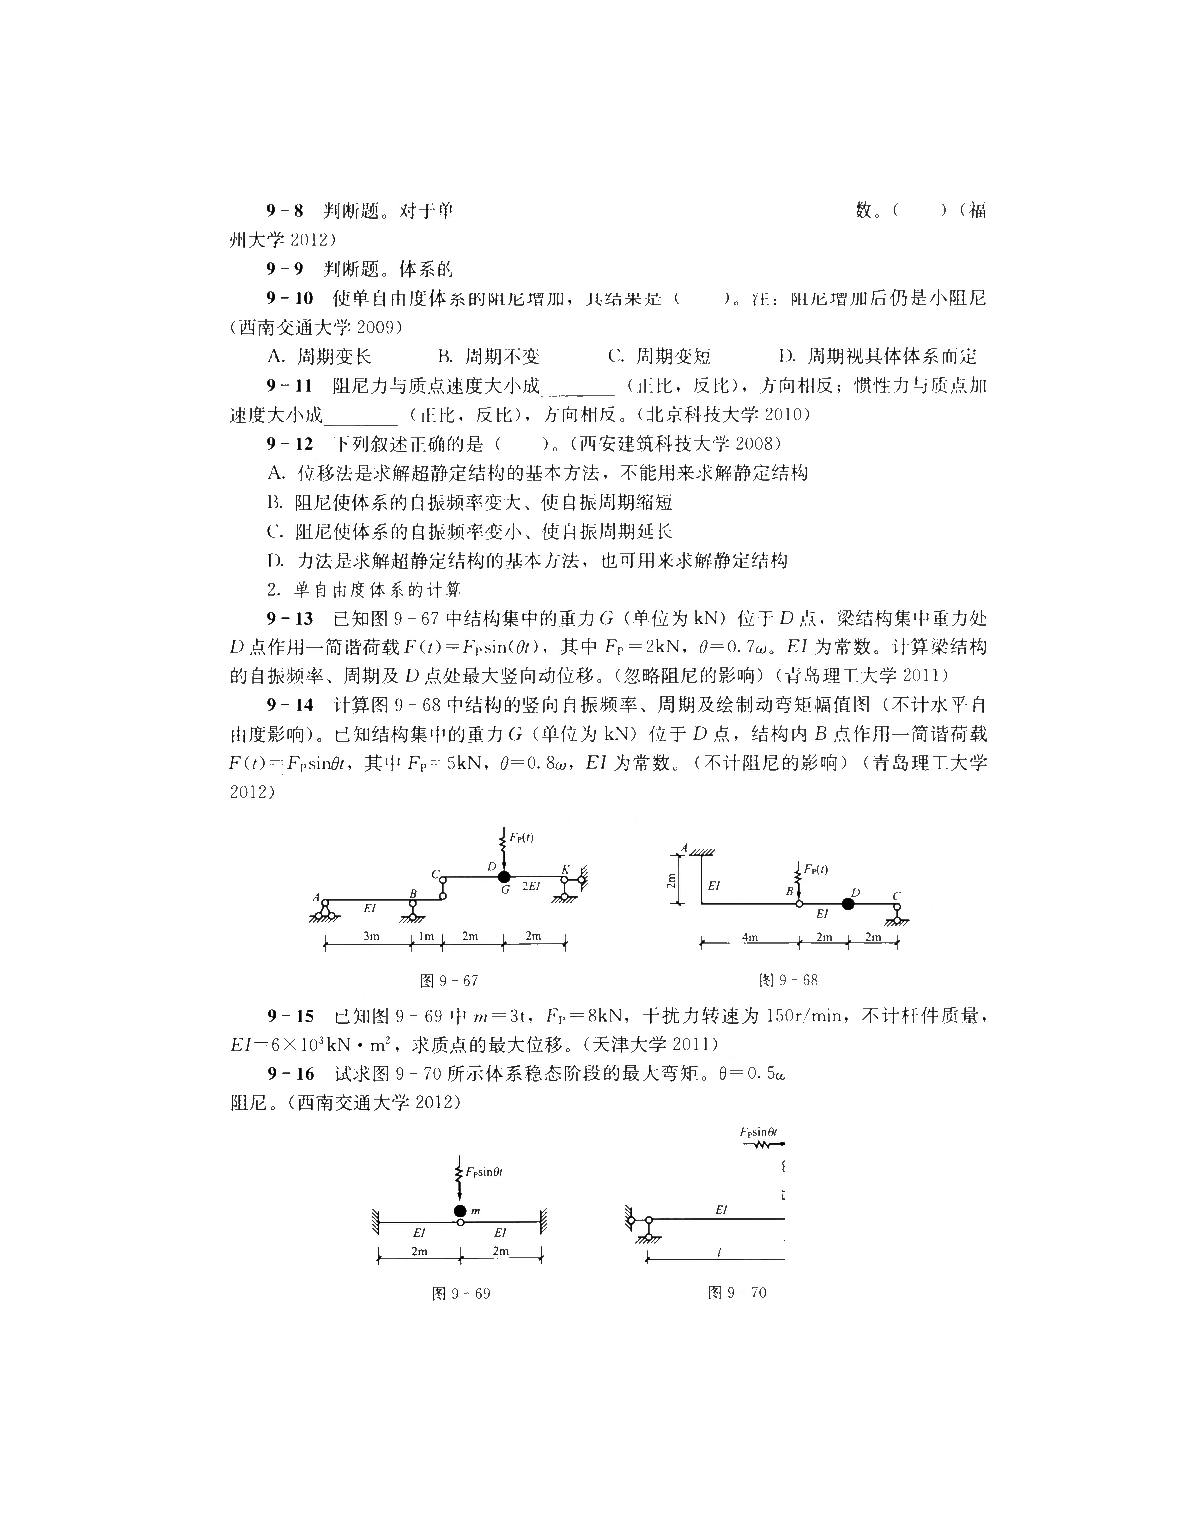
\includegraphics[width=0.92\textwidth]{figures/src18_p002.jpg}
\caption{结构力学基础与技巧班第15次作业及答案（动力学） 第 2 页清理图形页}
\end{figure}
\subsection*{第 3 页转写}
9-17图9-71所示结构承受简谐荷载Fpsinat的作用，设各柱EI相同，不计柱的质

5EI

量，不计阻尼。试求质量 的最大动位移。设6

（湖南大学2012)

9-18图9-72所示结构承受Fpsint简谐荷载的作用。各杆EI相同，不计杆的质量

和轴向变形，不计阻尼。设

/号，为结构的自振频率。试求：（1）体系的振动微分方

程；（2）质点m的振幅A。（重庆大学2009）

Fpsiner

Fsinet

图9-71

图9-72

3.多自由度体系的计算

9-19图9-73结构因横梁EI1=8，只能作反对称振动，试求其自振频率和主振型。

(81m1-)A+812m2A2=0

提示：两自由度结构自由振动振幅方程为

。（中南大学2010）

821mA +(82m2 -)

)A2=0

9-20建立图9-74所示结构的振动微分方程，并求解结构的自振频率和振型。（东南

大学2013)

El

2m

图9-73

图9-74

4.对称性的利用

9-21求图9-75所示体系的自振频率和主振型，EI=常数。（河北工业大学2012、

西南交通大学2008）

9-22试求图9-76所示对称体系的最低自振频率。EI=常数。（西南交通大学2012、

重庆大学2009类似)
\begin{figure}[H]\centering
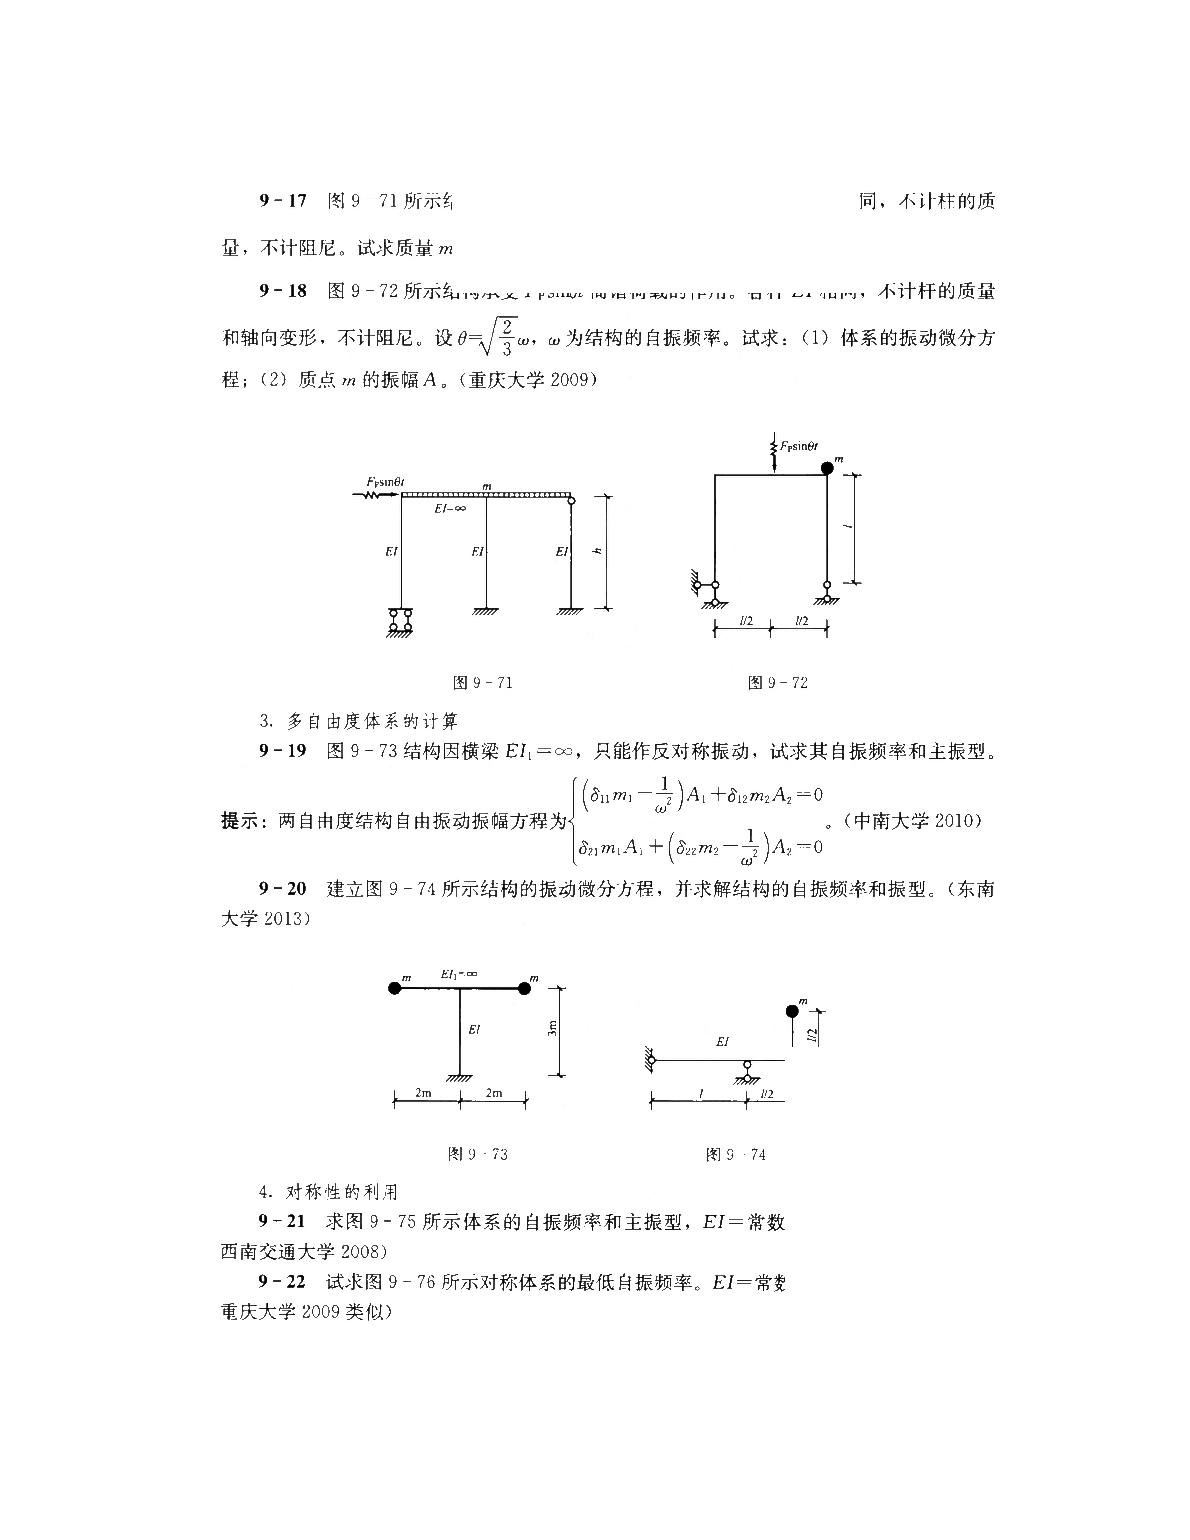
\includegraphics[width=0.92\textwidth]{figures/src18_p003.jpg}
\caption{结构力学基础与技巧班第15次作业及答案（动力学） 第 3 页清理图形页}
\end{figure}
\subsection*{第 4 页转写}
图9-75

图9-76

5.弹簧（支座）的计算

24EI

9-23图9-77（a）所示单跨梁的自振频率为

今在其集中质量m处加一

5ml3

竖向弹簧支承，如图9-77（b）所示，设弹簧的刚度系数为k，则图9-77（b）的自振频率

。（北京科技大学2009）

EI

EI

EI

(a)

(b)

图9-77

9-24求图9-78所示体系的自振频率。质量为m，各杆EI=常数，弹性支承的刚度

系数k=EI/13。（湖南大学2010)

9-25求图9-79所示结构的自振频率。（福州大学2008）

12

图9-78

图9-79

9-26试求图9-80所示体系的自振频率及质量m的最大动力位移，设0=0.5w，

弹簧刚度k=0.5EI/3，各杆的EI值相同，计算时不考虑阻尼影响。（清华大学2009）

Fpsingt

图9-80
\begin{figure}[H]\centering
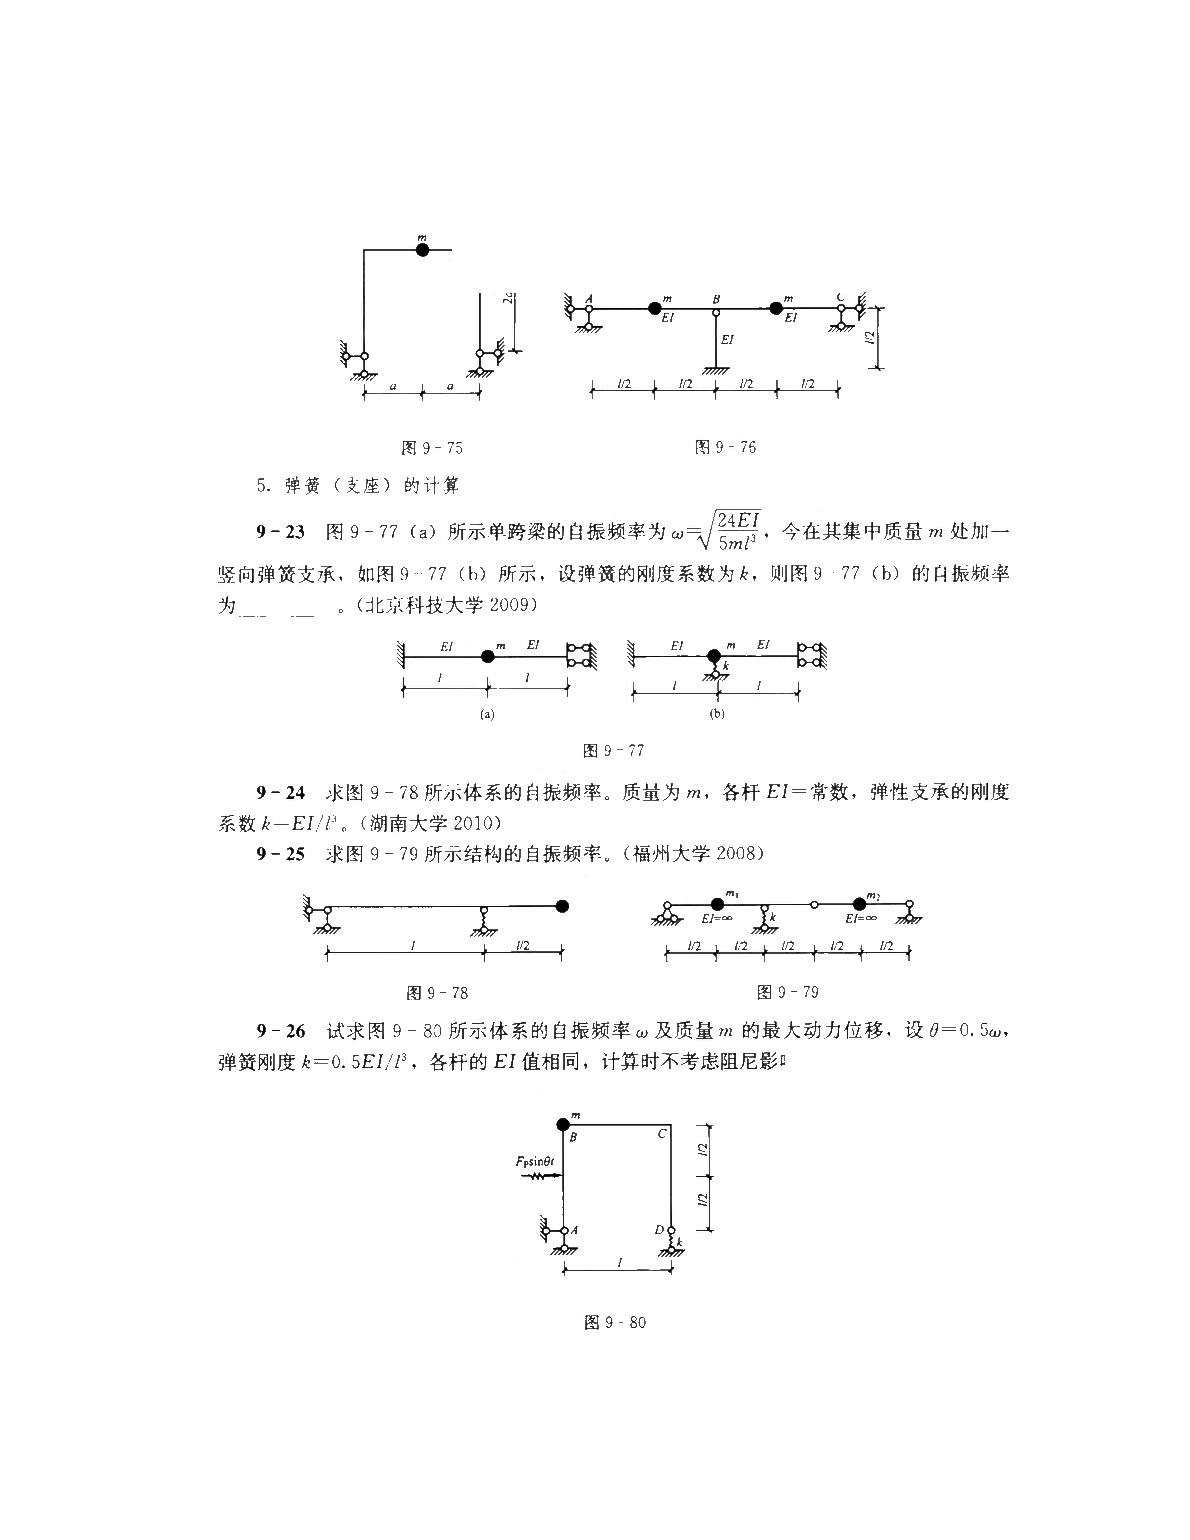
\includegraphics[width=0.92\textwidth]{figures/src18_p004.jpg}
\caption{结构力学基础与技巧班第15次作业及答案（动力学） 第 4 页清理图形页}
\end{figure}
\subsection*{第 5 页转写}
十二、练习题答案

9-1D。提示：增加的链杆数见图9-81。

9-22。提示：增加的链杆数见图9-82。

图9-81

图9-82

9-3

2.

9-4

9-5

C.

9-6

增大；减小。

9-7

X。提示：图9-66（a）的约束比图9-66（b）强，因此频率大。

9-8

X。提示：还应是简谐荷载且荷载作用在质量上。

9-9

X。提示：当》>w时，$\beta$0。

9-10

A.

9-11

正比；正比。

9-12

C.

Elg.

T=2元

3.92

9-13

EIg

动max

3EIg

44G

T=2元

9-14

动弯矩幅值图见图9-83。提示：本题实际上有两

44G

3EIg

个自由度，但题目要求不计水平自由度的影响，只考虑竖向惯性力，因此按单自由度体系求

解。$\beta$=2. 78, y(t)=370;7si

sinft.

EI

9-15

ymx=2.128mm。提示：w=38.73s-1，$\beta$=1.197。

9-16

Mmax=2Fpl/3。提示：$\beta$=4/3，M(t)=$\beta$Mstsinot。

Fph3

9-17

15EI

Ymex

提示：

10ET.

mh3，$\beta$=1.5。

3EI

3Fp/3

9-18

(1) (t)+号

32m

2ml3y(t)

16EI

9-19

假设水平振动方向为1方向（向右为正），竖直振动方向为2方向（向下为正）。

EI

Y1-0.847

Y12

第二振型为

第一振型为

wl=0.1596

1.18

w2=0.603

Y21
\begin{figure}[H]\centering
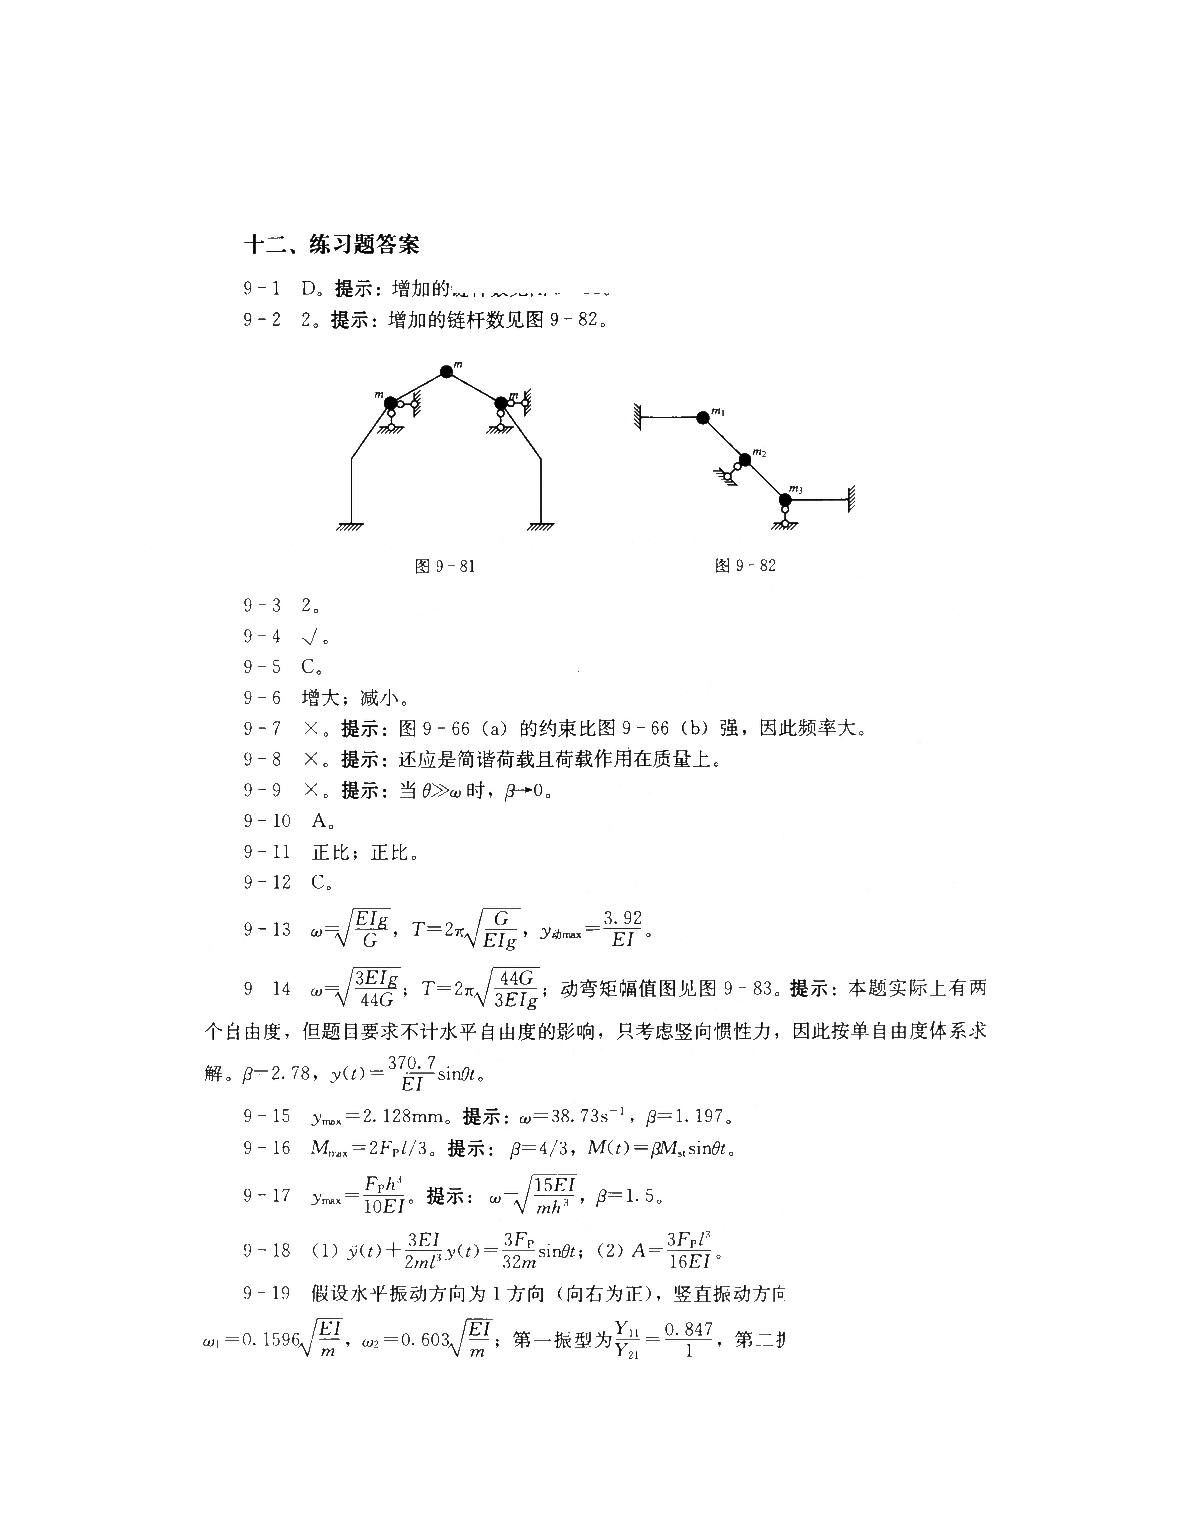
\includegraphics[width=0.92\textwidth]{figures/src18_p005.jpg}
\caption{结构力学基础与技巧班第15次作业及答案（动力学） 第 5 页清理图形页}
\end{figure}
\subsection*{第 6 页转写}
示：取反对称半结构见图9－84，有两个自由度，注意竖杆的刚度应减半，柔度系数m=

18

18

24

El,= 00

52.32

5kN

16.16kN

EI/2

52.32

16.16

动弯矩幅值图（单位：kN m)

反对称半结构

图9-83

图9-84

9-20假设水平振动方向为1方向（向右为正），竖向振动方向为2方向（向下为正）。

y(t)+mls

4E(t)+mls

48E)J2(t)=0

振动微分方程为

；自振频率=1.7

c2=5.89

7ml3

+(3) 3C

48E)i(2)+ml

8E)J2(t)=0

0.659

Y21

Y22

713

13

提示：柔度系数811

012

48ET

4EI

8E1$^\circ$

9-21假设水平振动方向为1方向（向右为正），竖直振动方向为2方向（向下为正），

120EI

求振型时不需要计算，可以根据振动的特点分析：由于反对称振型是第一振型，

1lma3。

Yn=1

此时质点沿水平振动，竖向位移为零，即第一振型为

Y21

Y12-

点竖向振动，其水平位移为零，因此第二振型为

Y22

48EI

9-22

提示：反对称半结构对应的自振频率低。

24EI+k

9-23

提示：可以看作弹簧并联。

5ml3

8EI

9-24

19ml3

16k

9-25

提示：本题为单自由度体系。

4ml+9m2

3EI

67Fp13

6713

9-26

8ml3;

Ymax
\begin{figure}[H]\centering
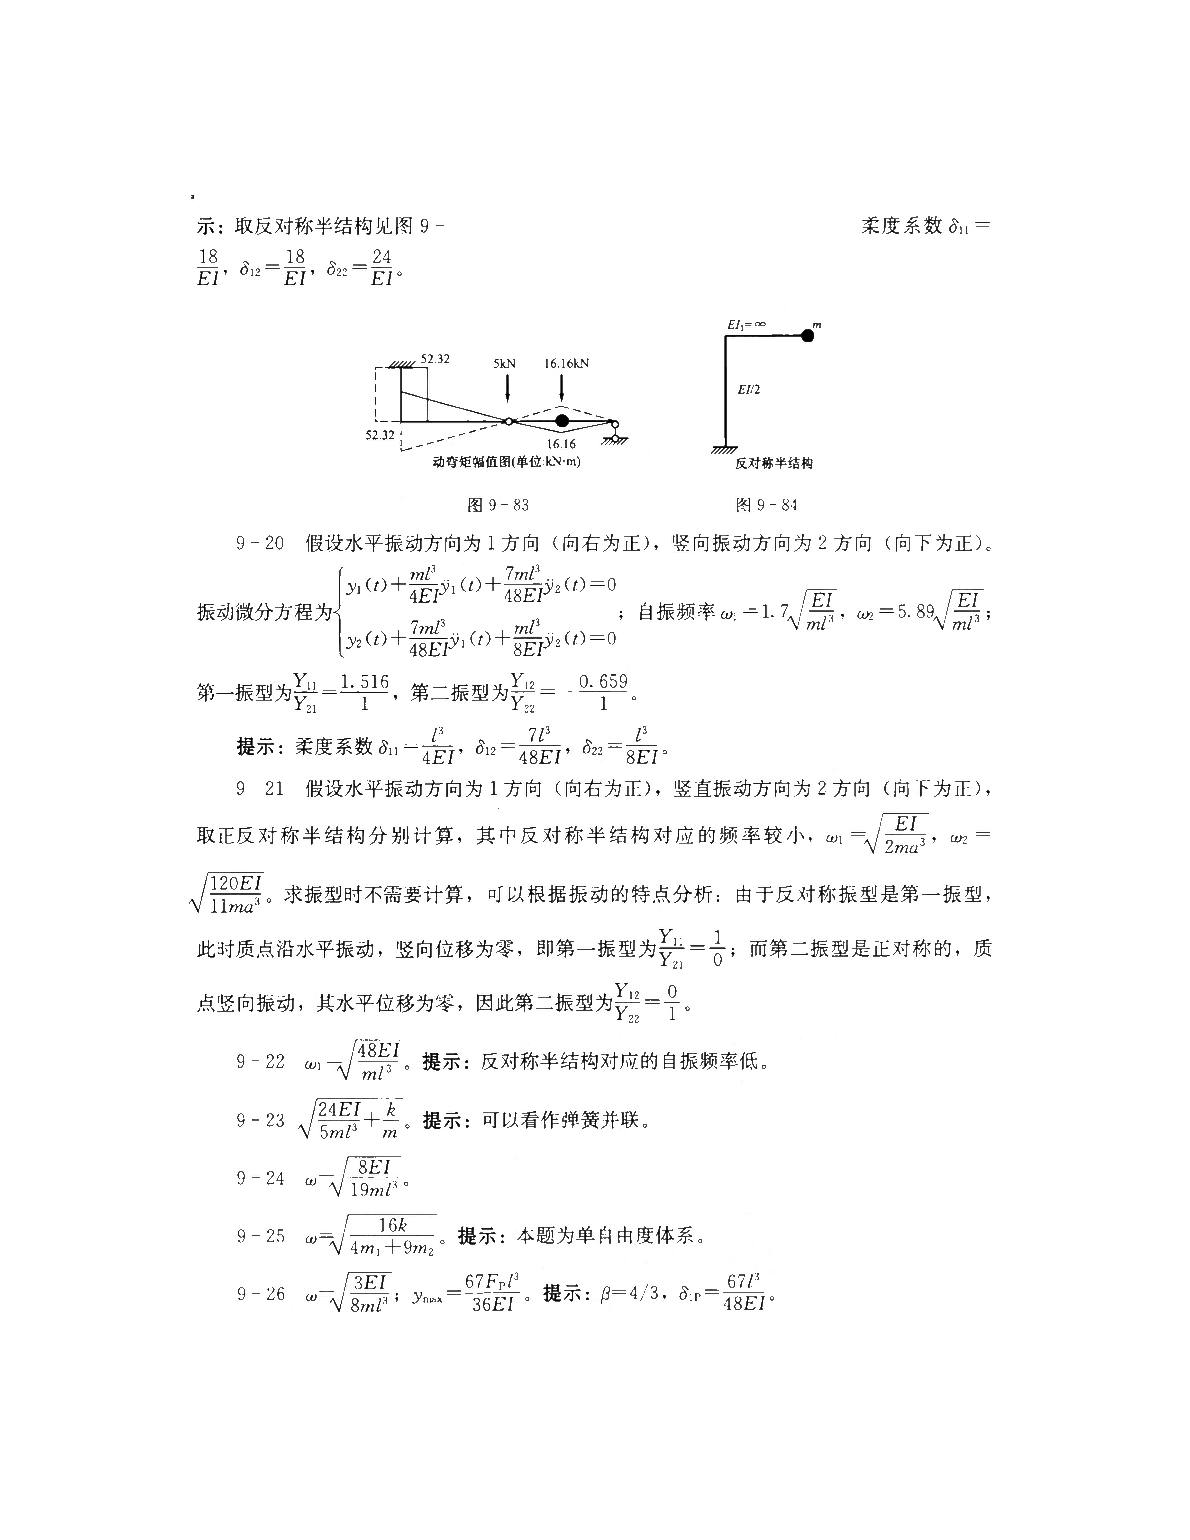
\includegraphics[width=0.92\textwidth]{figures/src18_p006.jpg}
\caption{结构力学基础与技巧班第15次作业及答案（动力学） 第 6 页清理图形页}
\end{figure}
